% =====================================================
\chapter{Literature Survey}
\label{chap:literature_survey}


This chapter builds the theoretical foundation for the work presented in this report.  
It traces the evolution of modern generative modeling from attention-based architectures such as Transformers~\cite{vaswani2017attention} and Vision Transformers~\cite{dosovitskiy2020vit} to early generative frameworks like GANs~\cite{goodfellow2014gan, karras2019stylegan} and VAEs~\cite{kingma2013autoencoding}, culminating in diffusion models that now dominate controllable image synthesis.  
The discussion then explores conditioning mechanisms, adapters, and perceptual style descriptors CLIP~\cite{radford2021clip}, IP-Adapter~\cite{chen2023ipadapter}, and CSD~\cite{somepalli2024csd} that make diffusion models both semantically and stylistically aware.  
The emphasis remains on clarity and intuition rather than exhaustive derivation.


% =====================================================
\section{Transformers: Attention-Based Sequence Modeling}
\label{sec:transformers}

Transformers~\cite{vaswani2017attention} revolutionized neural network design by discarding recurrence in favor of parallel attention.  
Every element of a sequence can attend to every other, learning global context in a single step.  
The self-attention mechanism is defined as:
\[
\mathrm{Attention}(Q,K,V)
=\mathrm{softmax}\!\Big(\frac{QK^\top}{\sqrt{d_k}}\Big)V, \qquad
Q=XW_Q,\;K=XW_K,\;V=XW_V.
\]
Residual connections and layer normalization stabilize deep stacks~\cite{vaswani2017attention}, while positional encodings supply sequence order.  
Transformers became the blueprint for multimodal systems such as CLIP~\cite{radford2021clip}, Stable Diffusion~\cite{rombach2022ldm}, and IP-Adapter~\cite{chen2023ipadapter}, where attention serves as the communication channel between modalities.  
Attention converts pairwise similarity into learnable weighting~\cite{vaswani2017attention}.  
In diffusion models, this same principle governs how textual or visual prompts “speak’’ to the U–Net~\cite{ronneberger2015unet} at each denoising step.


\begin{figure}[!htbp]
  \centering
  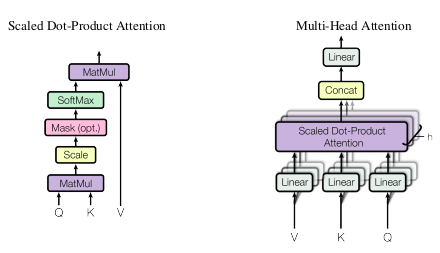
\includegraphics[width=0.75\linewidth]{images/transformer_attention.png}
  \caption{Self-attention pipeline: query–key similarity produces data-dependent mixing of values (adapted from Vaswani et al., 2017~\cite{vaswani2017attention}).}
  \label{fig:transformer_attention}
\end{figure}
\FloatBarrier


% =====================================================
\section{Vision Transformers (ViT)}
\label{sec:vit}

The Vision Transformer (ViT)~\cite{dosovitskiy2020vit} treats an image as a sequence of non-overlapping $P{\times}P$ patches that act as tokens.  
Each patch is linearly projected and combined with positional embeddings before passing through stacked transformer encoders.  
A [CLS] token aggregates global information for classification.

ViT removes locality bias and allows any patch to attend to any other, thereby capturing long-range dependencies such as fog gradients or underwater scattering, which are critical for environmental style modeling.

\begin{figure}[!htbp]
  \centering
  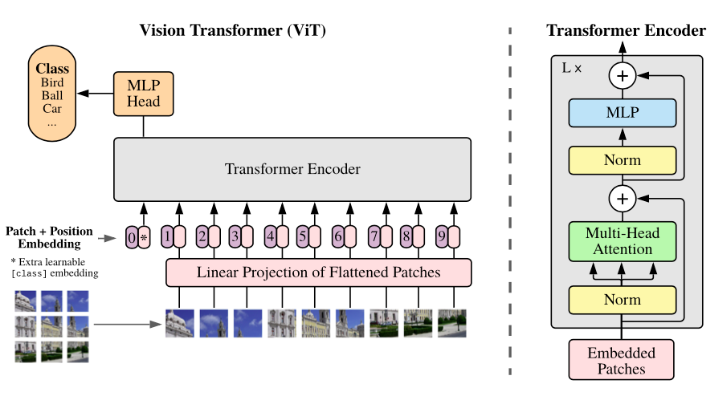
\includegraphics[width=0.75\linewidth]{images/vit_pipeline.png}
  \caption{ViT pipeline and Transformer Block (adapted from Dosovitskiy et al., 2021~\cite{dosovitskiy2020vit}).}
  \label{fig:vit_pipeline}
\end{figure}
\FloatBarrier


% =====================================================
\section{Generative Adversarial Networks (GANs)}
\label{sec:gans}

\textbf{Generative Adversarial Networks (GANs)}~\cite{goodfellow2014gan} were the first to produce high-fidelity synthetic images.  
They train a Generator $G$ and Discriminator $D$ in an adversarial loop:
\[
\min_G \max_D
\mathbb{E}_{x\sim p_\text{data}}[\log D(x)]
+\mathbb{E}_{z\sim p_z}[\log(1-D(G(z)))].
\]
GANs introduced sampling from a learned distribution rather than memorizing examples, but adversarial training often causes instability and mode collapse.  
Variants such as WGAN~\cite{arjovsky2017wassersteingan} and StyleGAN~\cite{karras2019stylegan} improved visual realism; however, they lacked semantic control and physical interpretability.

\begin{figure}[!htbp]
  \centering
  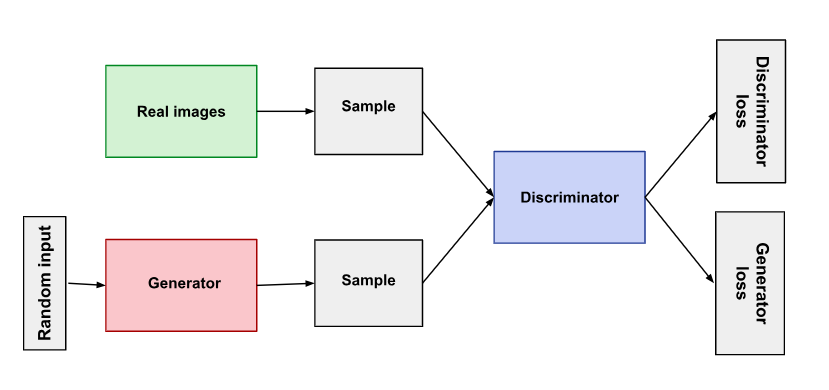
\includegraphics[width=0.72\linewidth]{images/gan_architecture.png}
  \caption{GAN architecture: generator–discriminator adversarial training loop (adapted from Foster, 2023~\cite{foster2023generativedeeplearning}).}
  \label{fig:gan_architecture}
\end{figure}

\FloatBarrier

% =====================================================
\section{Variational Autoencoders (VAEs)}
\label{sec:vaes}

VAEs~\cite{kingma2013autoencoding} model data generation via a continuous latent variable $z$.  
They maximize the Evidence Lower Bound (ELBO):
\[
\log p_\theta(x) \ge 
\mathbb{E}_{q_\phi(z|x)}[\log p_\theta(x|z)]
- \mathrm{KL}\!\big(q_\phi(z|x)\|p(z)\big),
\quad
z = \mu_\phi(x) + \sigma_\phi(x)\odot\epsilon.
\]
VAEs yield smooth, interpretable latent manifolds, enabling continuous interpolation between images.  
Although outputs can appear slightly blurred, VAEs provide stability and differentiable latent sampling, which are properties later exploited in Latent Diffusion Models (LDMs)~\cite{rombach2022ldm}.

\begin{figure}[!htbp]
  \centering
  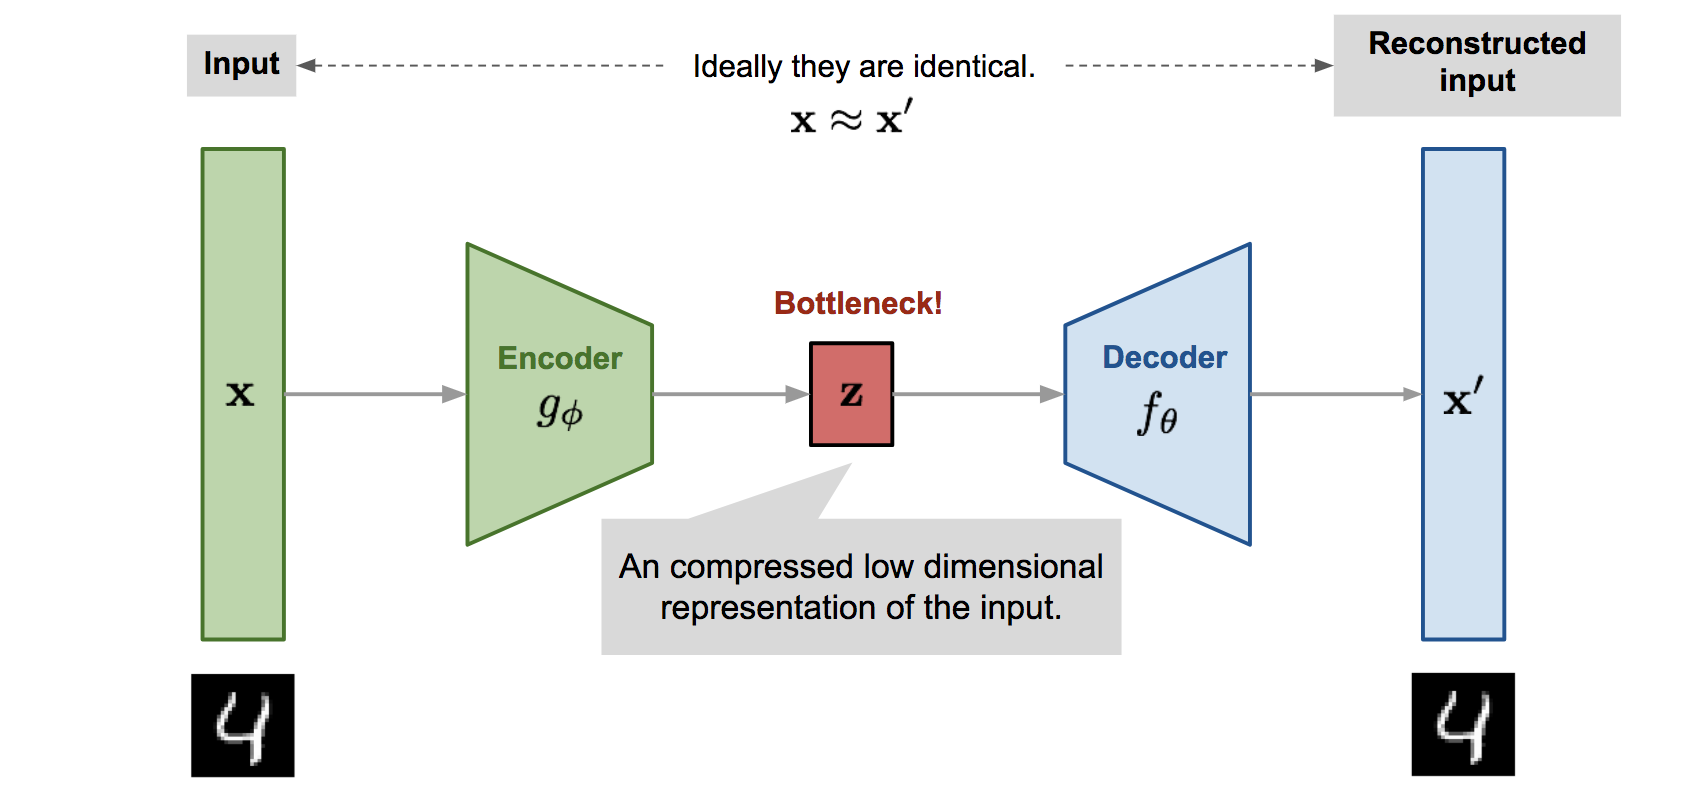
\includegraphics[width=0.75\linewidth]{images/vae_architecture.png}
  \caption{Variational Autoencoder: encoder–decoder with reparameterization trick (adapted from Foster, 2023~\cite{foster2023generativedeeplearning}).}
  \label{fig:vae_architecture}
\end{figure}

\FloatBarrier

% =====================================================
\section{U–Net Backbone for Vision and Diffusion}
\label{sec:unet}

U-Net~\cite {ronneberger2015unet} provides hierarchical feature extraction through an encoder–decoder architecture with skip connections that preserve fine detail.  
Diffusion models augment U–Net with \textbf{time-step embeddings} (representing noise level) and \textbf{cross-attention layers} (for text or image conditions), forming the structural engine of modern denoising diffusion.  
The encoder progressively downsamples the noisy image into coarse latent features, capturing global semantics, while the decoder reconstructs spatial details through upsampling operations.  
Skip connections ensure that high-frequency information from the encoder is directly passed to the corresponding decoder stage, preventing the loss of geometric or boundary details.  
Time-step embeddings allow the model to adjust its denoising strength dynamically—focusing on coarse structure during early steps and fine details in later stages.  
Cross-attention integrates contextual guidance, enabling the model to align visual content with prompts, reference styles, or other conditioning inputs.  
This combination of hierarchical reconstruction, temporal awareness, and multimodal conditioning makes U–Net a robust backbone for diffusion-based image synthesis and environmental style transfer.

\begin{figure}[!h]
  \centering
  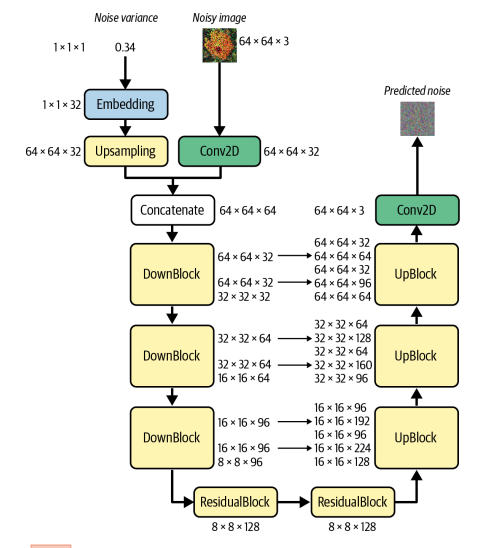
\includegraphics[width=0.60\linewidth]{images/unet_architecture.png}
  \caption{Diffusion U–Net: encoder–decoder with skip connections, time-step embeddings, and cross-attention (adapted from Foster, 2023~\cite{foster2023generativedeeplearning}).}
  \label{fig:unet_architecture}
\end{figure}
\FloatBarrier

% =====================================================
\section{Diffusion Models: From Noise to Structure}
\label{sec:diffusion_models}

Diffusion models~\cite{ho2020ddpm} constitute a family of generative models that gradually convert pure noise into structured data through a learned denoising process.  
They interpret image generation as the reversal of a known stochastic diffusion—a physically inspired process analogous to entropy reduction.

\subsection*{Forward (Noising) Process}

The forward process progressively destroys image structure by adding Gaussian noise over $T$ discrete timesteps according to a variance schedule $\{\beta_t\}_{t=1}^T$.  
Starting from a clean image $x_0$, each step produces a noisier version:
\[
q(x_t|x_{t-1})=\mathcal{N}\big(\sqrt{1-\beta_t}\,x_{t-1},\,\beta_t I\big).
\]
Iterating this process yields a closed form for any timestep $t$:
\[
x_t = \sqrt{\bar{\alpha}_t}\,x_0 + \sqrt{1-\bar{\alpha}_t}\,\epsilon,
\quad
\bar{\alpha}_t = \prod_{i=1}^t (1-\beta_i),
\]
where $\epsilon\sim\mathcal{N}(0,I)$ represents random Gaussian noise.  
As $t\!\to\!T$, $\bar{\alpha}_t\!\to\!0$ and $x_T$ approaches pure noise, meaning all information about $x_0$ is effectively lost.

This stage mimics a physical diffusion process, where structured data dissolves into randomness.  
The corruption is fully known and mathematically invertible, allowing the model to learn the reverse process.

\begin{figure}[!htbp]
  \centering
  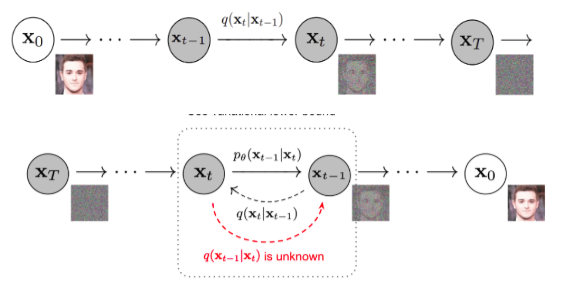
\includegraphics[width=0.75\linewidth]{images/ddpm_forward_reverse.png}
  \caption{Forward and reverse diffusion: corruption by Gaussian noise and stepwise denoising (adapted from Foster, 2023~\cite{foster2023generativedeeplearning}).}
  \label{fig:diffusion_process}
\end{figure}
\FloatBarrier

\subsection*{Reverse (Denoising) Process}

The reverse process attempts to invert the corruption and reconstruct the data distribution.  
A neural network $\epsilon_\theta(x_t,t)$ is trained to predict the noise component at each timestep.  
Given $x_t$, the model estimates $\epsilon_\theta$ and computes the mean of the reverse conditional:
\[
p_\theta(x_{t-1}|x_t)
=\mathcal{N}\!\big(\mu_\theta(x_t,t),\,\sigma_t^2 I\big),
\quad
\mu_\theta(x_t,t)=\frac{1}{\sqrt{1-\beta_t}}
\Big(x_t-\frac{\beta_t}{\sqrt{1-\bar{\alpha}_t}}\,\epsilon_\theta(x_t,t)\Big).
\]
Training minimizes the denoising objective:
\[
\mathcal{L}_{\text{simple}}
=\mathbb{E}_{x_0,t,\epsilon}
\big[\|\epsilon-\epsilon_\theta(\sqrt{\bar{\alpha}_t}x_0+\sqrt{1-\bar{\alpha}_t}\epsilon,t)\|^2\big].
\]

\paragraph{Sampling.}
At inference, the process begins from random noise $x_T\!\sim\!\mathcal{N}(0,I)$ and iteratively applies
\[
x_{t-1} = \frac{1}{\sqrt{1-\beta_t}}
\Big(x_t - \frac{\beta_t}{\sqrt{1-\bar{\alpha}_t}}\,\epsilon_\theta(x_t,t)\Big)
+ \sigma_t z, \qquad z\sim\mathcal{N}(0,I),
\]
until $x_0$ emerges.  
Each denoising step restores a small fraction of structure, producing interpretable evolution from pure noise to a coherent image.

\subsection*{Observations}

Diffusion can be understood as \textit{entropy minimization} or \textit{energy descent}.  
The forward process increases entropy (information destruction), while the learned reverse process systematically decreases it, similar to annealing a chaotic physical system back into order.  
This stepwise refinement makes diffusion both stable and explainable compared to GANs or VAEs.

\paragraph{Key Properties.}
\begin{itemize}
  \item \textbf{Stability:} Training minimizes a single, convex denoising objective, avoiding adversarial instability.
  \item \textbf{Interpretability:} Intermediate latents correspond to partially denoised states, revealing the generative trajectory.
  \item \textbf{Controllability:} External conditions (e.g., text, depth, style) can guide the reverse process at every step.
\end{itemize}

These properties make diffusion the most physically grounded and perceptually faithful generative paradigm, forming the basis for architectures such as Stable Diffusion~\cite{rombach2022ldm}, ControlNet~\cite{zhang2023controlnet}, and the proposed      CSD-guided models in this work.

% =====================================================
\section{Conditional and Guided Diffusion}
\label{sec:conditional_diffusion}

To steer generation, diffusion can incorporate conditioning variables.

\paragraph{Classifier-Based Guidance.}
In this implementation \cite{dhariwal2021diffusion} an external classifier $p_\phi(y|x_t)$ trained on noisy images guides sampling by adjusting the predicted noise:
\[
\tilde{\epsilon}_\theta(x_t,t|y)
=\epsilon_\theta(x_t,t)
- w\,\sigma_t\nabla_{x_t}\log p_\phi(y|x_t),
\]
where $w$ scales guidance strength.  
This approach ensures class consistency but adds complexity and gradient noise.

\paragraph{Cross-Attention Conditioning.}
Modern diffusion integrates conditioning directly inside the U–Net~\cite {ronneberger2015unet}:
\[
\text{CrossAttn}(Q,K,V)=
\text{softmax}\!\Big(\frac{QK^\top}{\sqrt{d_k}}\Big)V,
\]
with $(K,V)$ from attention based~\cite{vaswani2017attention} conditioning encoders (text or style) and $Q$ from U–Net activations.  
This mechanism allows natural language or reference images to guide generation internally, forming the foundation of controllable diffusion.

\FloatBarrier

% =====================================================
\section{Latent Diffusion and Stable Diffusion}
\label{sec:ldm_stable}

Latent Diffusion Models (LDMs)~\cite{rombach2022ldm} perform diffusion in the latent space of a pretrained VAE, drastically reducing computation.  
\textbf{Stable Diffusion}~\cite{podell2023sdxl} extends this concept by injecting CLIP~\cite{radford2021clip} text embeddings via cross-attention, achieving text-to-image synthesis with photorealistic fidelity.

Operating in latent space focuses on perceptually relevant features.  
The text encoder becomes a compass that steers denoising toward the prompt description (for instance, “foggy valley’’ or “snow-covered forest’’).

\begin{figure}[!htbp]
  \centering
  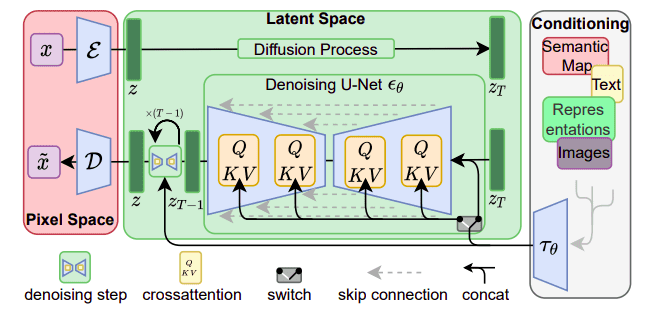
\includegraphics[width=0.7\linewidth]{images/stable_diffusion_architecture.png}
  \caption{Stable Diffusion: text-conditioned latent denoising within a VAE encoder–decoder pipeline (adapted from Foster, 2023~\cite{foster2023generativedeeplearning}).}
  \label{fig:stable_diffusion}
\end{figure}

\FloatBarrier

% =====================================================
\section{Contrastive Learning and CLIP Encoders}
\label{sec:contrastive_clip}

Contrastive learning aligns images and text in a shared embedding space.  
CLIP~\cite{radford2021clip} employs dual encoders trained with the Information Noise-Contrastive Estimation loss:
\[
\mathcal{L}_{\text{CLIP}}
=-\frac{1}{N}\sum_{i=1}^N
\Big[
\log\frac{e^{v_i^\top t_i/\tau}}{\sum_j e^{v_i^\top t_j/\tau}}
+\log\frac{e^{v_i^\top t_i/\tau}}{\sum_j e^{v_j^\top t_i/\tau}}
\Big].
\]
Matching image–text pairs obtain high cosine similarity, giving diffusion linguistic grounding.  
However, CLIP conflates semantics and style, motivating newer decoupled adapters.

\begin{figure}[!htbp]
  \centering
  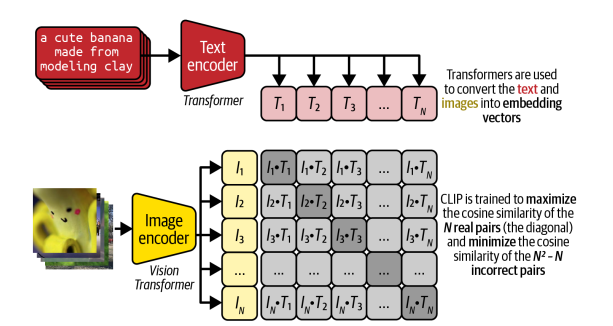
\includegraphics[width=0.65\linewidth]{images/clip_contrastive.png}
  \caption{CLIP: contrastive alignment between image and text embeddings (adapted from Foster, 2023~\cite{foster2023generativedeeplearning}).}
  \label{fig:clip_contrastive}
\end{figure}

\FloatBarrier

% =====================================================
\section{CSD: Contrastive Style Descriptors}
\label{sec:csd}

Contrastive Style Descriptors (CSD)~\cite{somepalli2024csd} define a perceptual embedding space purely for style.  
A ViT backbone learns to pull together stylistically similar pairs and push apart dissimilar ones.  
Similarity is computed as:
\[
\mathrm{Sim}(x_g,x_r)=
\frac{z_g^\top z_r}{\|z_g\|\|z_r\|}.
\]
Unlike CLIP, CSD is content-invariant, capturing stylistic attributes such as haze intensity or lighting tone.  
In diffusion, a frozen CSD encoder can serve as a perceptual critic, aligning generated samples to the target style manifold.

If CLIP aligns “meaning,’’ CSD aligns “feel.’’  
It measures how similar two images are in mood or visual atmosphere, thereby enabling perceptually guided diffusion.

% =====================================================
\section{Adapters, Structural Guidance, and Prompt Fusion}
\label{sec:adapters_control}

Adapters add modular control to pretrained diffusion models.  

\textbf{ControlNet}~\cite{zhang2023controlnet} introduces a zero-initialized side network that processes structural cues (e.g., edges or depth) and merges them back into the U–Net to preserve geometry.  
It enables pixel-accurate layout control while maintaining stability.  
ControlNet acts as a geometry channel that learns to modulate generation based on structural hints such as sketch-to-image or depth-aware synthesis.  
The side network mirrors the layers of the main U–Net, ensuring that spatial information flows consistently across scales without disturbing the pretrained diffusion backbone.  
Because the parameters are initialized to zero, the model begins as an exact copy of the base diffusion system and gradually learns to incorporate external structure only when relevant.  
This design prevents training instability and allows seamless integration of structural control without sacrificing prior semantic alignment.  
By conditioning on cues like canny edges, segmentation maps, or normal maps, ControlNet ensures that generated outputs adhere closely to desired spatial layouts while preserving natural texture and lighting.  
Its modular nature also allows multiple conditioning types—such as depth, pose, or scribbles—to be fused simultaneously, enabling precise and interpretable control over the generative process.

\begin{figure}[!htbp]
  \centering
  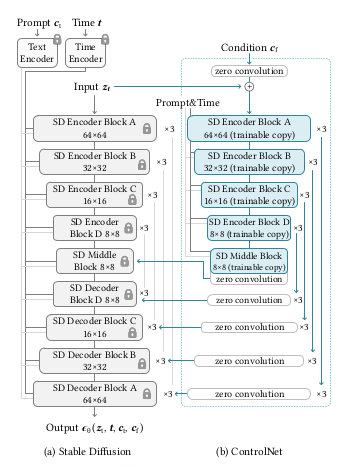
\includegraphics[width=0.7\linewidth]{images/controlnet_architecture.png}
  \caption{ControlNet: structure encoder merged into U–Net via additive connections (adapted from Zhang et al., 2023~\cite{zhang2023controlnet}).}
  \label{fig:controlnet_architecture}
\end{figure}

\FloatBarrier

\textbf{IP-Adapter}~\cite{chen2023ipadapter} adds an image encoder whose embeddings are injected through decoupled cross-attention alongside text embeddings.  
InstantStyle~\cite{wang2024instantstyle} further refines this by subtracting the text-projected component of the image embedding, leaving a \emph{style residual} for targeted appearance injection.  
This residual ensures that the visual information contributes only stylistic cues—such as color tone, illumination, and material texture—while preventing semantic interference from the reference image.  
In the diffusion U–Net, the IP-Adapter’s embeddings act as additional key–value pairs in cross-attention, influencing feature activations at selective layers where appearance dominates (typically early upsampling blocks).  
By decoupling semantics from appearance, the model can adapt the “look’’ of the generated scene while retaining the prompt’s original structure and composition.  
This modular mechanism enables efficient and training-free personalization, allowing diffusion models to mimic a given visual domain (fog, underwater, dusk) simply by conditioning on a single reference image.  
Text dictates “what’’ to draw, whereas the reference image defines “how’’ it should appear—controlling tone, color, and texture without disturbing geometry or content alignment.

\begin{figure}[!htbp]
  \centering
  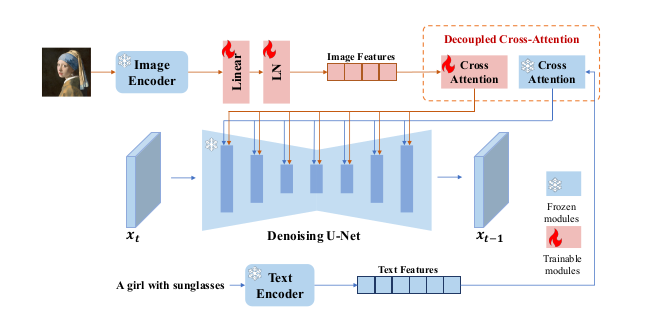
\includegraphics[width=0.7\linewidth]{images/ip_adapter_architecture.png}
  \caption{IP-Adapter: decoupled attention merges text semantics and image-based style cues (adapted from Chen et al., 2023~\cite{chen2023ipadapter}).}
  \label{fig:ip_adapter_architecture}
\end{figure}

\FloatBarrier

% =====================================================
\section*{Summary}

Research has steadily advanced toward controllable and interpretable generation.  
Transformers introduced attention mechanisms, ViTs extended them to vision, and GANs and VAEs pioneered generative modeling.  
Diffusion unified these ideas into a stable probabilistic framework, enhanced by latent conditioning, cross-attention, and adapters like ControlNet and IP-Adapter.  
Contrastive systems such as CLIP and CSD added semantic and stylistic grounding, forming the basis for the adaptive, CSD-guided diffusion explored here.
